% Week 1: Course Introduction
% CSI403 Full Stack Development
\documentclass[aspectratio=169,11pt]{beamer}

\usetheme{Madrid}
\usecolortheme{default}
\setbeamertemplate{navigation symbols}{}

\usepackage[T1]{fontenc}
\usepackage{tikz}
\usepackage{booktabs}

\definecolor{maincolor}{RGB}{128,0,0}
\setbeamercolor{structure}{fg=maincolor}

\title{Week 1: Course Introduction}
\subtitle{CSI403 Full Stack Development}
\date{Semester 1/2569}

\begin{document}

\begin{frame}
    \titlepage
\end{frame}

\begin{frame}{Agenda}
    \tableofcontents
\end{frame}

%========================================
\section{Course Overview}
%========================================

\begin{frame}{Course Information}
    \begin{center}
        \begin{tabular}{ll}
            \toprule
            \textbf{Item} & \textbf{Detail} \\
            \midrule
            Course Code & CSI403 \\
            Course Name & Full Stack Development \\
            Credits & 3 (2-3-5) \\
            Semester & 1/2569 \\
            Duration & 15 weeks \\
            \bottomrule
        \end{tabular}
    \end{center}
\end{frame}

\begin{frame}{Important Notes}
    \begin{center}
        \Large
        \textbf{No Midterm Exam!}
        
        \vspace{0.5cm}
        
        \textbf{No Final Exam!}
        
        \vspace{1cm}
        
        \normalsize
        Assessment is based on:
        
        \vspace{0.3cm}
        
        \textbf{8 Labs (64\%) + Group Project (36\%)}
    \end{center}
\end{frame}

\begin{frame}{Two-Phase Learning Model}
    \begin{center}
        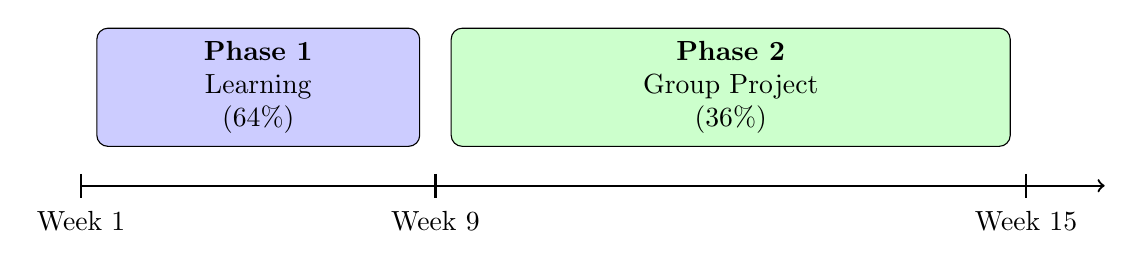
\begin{tikzpicture}
            % Timeline
            \draw[thick, ->] (0,0) -- (13,0);
            
            % Week markers
            \foreach \x/\w in {0/1, 4.5/9, 12/15} {
                \draw[thick] (\x,0.15) -- (\x,-0.15);
                \node[below] at (\x,-0.2) {Week \w};
            }
            
            % Phase 1 box
            \draw[fill=blue!20, rounded corners] (0.2,0.5) rectangle (4.3,2);
            \node[align=center] at (2.25,1.25) {\textbf{Phase 1}\\Learning\\(64\%)};
            
            % Phase 2 box
            \draw[fill=green!20, rounded corners] (4.7,0.5) rectangle (11.8,2);
            \node[align=center] at (8.25,1.25) {\textbf{Phase 2}\\Group Project\\(36\%)};
        \end{tikzpicture}
    \end{center}
\end{frame}

\begin{frame}{Phase 1: Learning (Week 2-9)}
    \textbf{Build TaskFlow System Together}
    
    \vspace{0.5cm}
    
    \begin{itemize}
        \item Learn by building a real application
        \item 8 weekly labs (8\% each)
        \item Guided step-by-step instructions
        \item Individual work
    \end{itemize}
    
    \vspace{0.5cm}
    
    \textbf{Total: 64\% of course grade}
\end{frame}

\begin{frame}{Phase 2: Group Project (Week 10-15)}
    \textbf{Apply What You Learned}
    
    \vspace{0.5cm}
    
    \begin{itemize}
        \item Form teams of 3-4 students
        \item Choose your own project idea
        \item Use all technologies from Phase 1
        \item Present and defend your work
    \end{itemize}
    
    \vspace{0.5cm}
    
    \textbf{Total: 36\% of course grade}
\end{frame}

%========================================
\section{Assessment}
%========================================

\begin{frame}{Phase 1 Assessment (64\%)}
    \begin{center}
        \begin{tabular}{clc}
            \toprule
            \textbf{Lab} & \textbf{Topic} & \textbf{Weight} \\
            \midrule
            Lab 1 & Git + Python + Setup & 8\% \\
            Lab 2 & FastAPI CRUD & 8\% \\
            Lab 3 & Database Integration & 8\% \\
            Lab 4 & Frontend Basics & 8\% \\
            Lab 5 & Jinja2 Templates & 8\% \\
            Lab 6 & Docker + Compose & 8\% \\
            Lab 7 & Testing + Jenkins CI & 8\% \\
            Lab 8 & Jenkins CD & 8\% \\
            \midrule
            & \textbf{Total} & \textbf{64\%} \\
            \bottomrule
        \end{tabular}
    \end{center}
\end{frame}

\begin{frame}{Phase 2 Assessment (36\%)}
    \begin{center}
        \begin{tabular}{clc}
            \toprule
            \textbf{Week} & \textbf{Deliverable} & \textbf{Weight} \\
            \midrule
            10 & G1: Project Proposal & 5\% \\
            11 & G2: System Design & 5\% \\
            12 & Checkpoint Demo & 8\% \\
            15 & Final Project & 12\% \\
            15 & Oral Defense & 4\% \\
            15 & Peer Evaluation & 2\% \\
            \midrule
            & \textbf{Total} & \textbf{36\%} \\
            \bottomrule
        \end{tabular}
    \end{center}
\end{frame}

\begin{frame}{Late Submission Policy}
    \begin{center}
        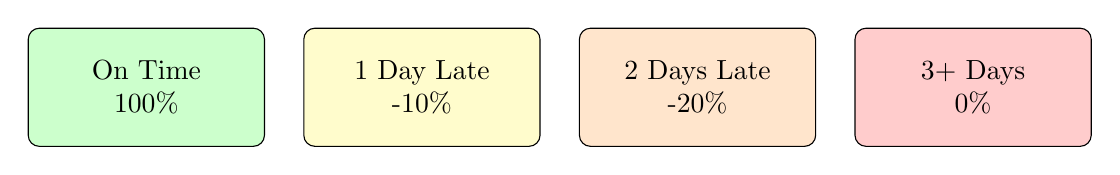
\begin{tikzpicture}
            \draw[fill=green!20, rounded corners] (0,0) rectangle (3,1.5);
            \node[align=center] at (1.5,0.75) {On Time\\100\%};
            
            \draw[fill=yellow!20, rounded corners] (3.5,0) rectangle (6.5,1.5);
            \node[align=center] at (5,0.75) {1 Day Late\\-10\%};
            
            \draw[fill=orange!20, rounded corners] (7,0) rectangle (10,1.5);
            \node[align=center] at (8.5,0.75) {2 Days Late\\-20\%};
            
            \draw[fill=red!20, rounded corners] (10.5,0) rectangle (13.5,1.5);
            \node[align=center] at (12,0.75) {3+ Days\\0\%};
        \end{tikzpicture}
    \end{center}
    
    \vspace{0.5cm}
    
    \begin{itemize}
        \item Deadline: Every Sunday 23:59
        \item Maximum 3 days late submission
        \item After 3 days = 0 points
    \end{itemize}
\end{frame}

%========================================
\section{TaskFlow System}
%========================================

\begin{frame}{Case Study: TaskFlow}
    \begin{center}
        \Large
        \textbf{Task Management System}
        
        \vspace{0.5cm}
        
        \normalsize
        A web application for managing tasks and to-do items
    \end{center}
    
    \vspace{0.5cm}
    
    Similar to: Todoist, Microsoft To-Do, Trello
\end{frame}

\begin{frame}{TaskFlow Features}
    \begin{columns}[T]
        \begin{column}{0.48\textwidth}
            \textbf{User Management:}
            \begin{itemize}
                \item User Registration
                \item Login / Logout
                \item Password Hashing
                \item Session Management
            \end{itemize}
        \end{column}
        \begin{column}{0.48\textwidth}
            \textbf{Task Management:}
            \begin{itemize}
                \item Create / Read / Update / Delete
                \item Status: Pending, In Progress, Done
                \item Priority: Low, Medium, High
                \item Categories
            \end{itemize}
        \end{column}
    \end{columns}
\end{frame}

\begin{frame}{TaskFlow Features (continued)}
    \begin{columns}[T]
        \begin{column}{0.48\textwidth}
            \textbf{Dashboard:}
            \begin{itemize}
                \item Task Statistics
                \item Recent Tasks
                \item Filter by Status
                \item Search Tasks
            \end{itemize}
        \end{column}
        \begin{column}{0.48\textwidth}
            \textbf{DevOps:}
            \begin{itemize}
                \item Docker Containers
                \item Docker Compose
                \item Automated Testing
                \item CI/CD Pipeline
            \end{itemize}
        \end{column}
    \end{columns}
\end{frame}

\begin{frame}{Database Schema}
    \begin{center}
        \begin{tikzpicture}[
            box/.style={draw, fill=##1, minimum width=3cm, minimum height=2cm, align=center, rounded corners}
        ]
            % Users table
            \node[box=blue!20] (users) at (0,0) {
                \textbf{Users}\\[0.2cm]
                id\\username\\email\\password
            };
            
            % Tasks table
            \node[box=green!20] (tasks) at (6,0) {
                \textbf{Tasks}\\[0.2cm]
                id\\title\\status\\user\_id
            };
            
            % Categories table
            \node[box=orange!20] (cats) at (12,0) {
                \textbf{Categories}\\[0.2cm]
                id\\name\\color
            };
            
            % Relationships
            \draw[->, thick] (users.east) -- node[above] {1 : N} (tasks.west);
            \draw[->, thick] (cats.west) -- node[above] {1 : N} (tasks.east);
        \end{tikzpicture}
    \end{center}
\end{frame}

%========================================
\section{Technology Stack}
%========================================

\begin{frame}{Technology Stack Overview}
    \begin{center}
        \begin{tikzpicture}[
            layer/.style={draw, fill=##1, minimum width=10cm, minimum height=1.2cm, align=center}
        ]
            \node[layer=blue!20] at (0,4) {\textbf{Frontend:} HTML, CSS, JavaScript, Bootstrap 5};
            \node[layer=green!20] at (0,2.5) {\textbf{Backend:} Python, FastAPI, Jinja2};
            \node[layer=orange!20] at (0,1) {\textbf{Database:} Microsoft SQL Server};
            \node[layer=red!20] at (0,-0.5) {\textbf{DevOps:} Docker, Jenkins, Git};
        \end{tikzpicture}
    \end{center}
\end{frame}

\begin{frame}{Frontend Technologies}
    \begin{columns}[T]
        \begin{column}{0.3\textwidth}
            \textbf{HTML5}
            \begin{itemize}
                \item Structure
                \item Semantic tags
                \item Forms
            \end{itemize}
        \end{column}
        \begin{column}{0.3\textwidth}
            \textbf{CSS3}
            \begin{itemize}
                \item Styling
                \item Flexbox
                \item Responsive
            \end{itemize}
        \end{column}
        \begin{column}{0.3\textwidth}
            \textbf{Bootstrap 5}
            \begin{itemize}
                \item Components
                \item Grid System
                \item Utilities
            \end{itemize}
        \end{column}
    \end{columns}
\end{frame}

\begin{frame}{Backend Technologies}
    \begin{columns}[T]
        \begin{column}{0.3\textwidth}
            \textbf{Python 3.11+}
            \begin{itemize}
                \item Modern syntax
                \item Type hints
                \item Async support
            \end{itemize}
        \end{column}
        \begin{column}{0.3\textwidth}
            \textbf{FastAPI}
            \begin{itemize}
                \item REST API
                \item Auto docs
                \item Validation
            \end{itemize}
        \end{column}
        \begin{column}{0.3\textwidth}
            \textbf{SQLAlchemy}
            \begin{itemize}
                \item ORM
                \item Migrations
                \item Relationships
            \end{itemize}
        \end{column}
    \end{columns}
\end{frame}

\begin{frame}{DevOps Technologies}
    \begin{columns}[T]
        \begin{column}{0.3\textwidth}
            \textbf{Docker}
            \begin{itemize}
                \item Containers
                \item Images
                \item Compose
            \end{itemize}
        \end{column}
        \begin{column}{0.3\textwidth}
            \textbf{Jenkins}
            \begin{itemize}
                \item CI/CD
                \item Pipelines
                \item Automation
            \end{itemize}
        \end{column}
        \begin{column}{0.3\textwidth}
            \textbf{Git/GitHub}
            \begin{itemize}
                \item Version control
                \item Branching
                \item Pull requests
            \end{itemize}
        \end{column}
    \end{columns}
\end{frame}

%========================================
\section{Schedule}
%========================================

\begin{frame}{Phase 1 Schedule (Week 1-9)}
    \begin{center}
        \small
        \begin{tabular}{cll}
            \toprule
            \textbf{Week} & \textbf{Topic} & \textbf{Lab} \\
            \midrule
            1 & Course Introduction & - \\
            2 & Git + Python + Setup & Lab 1 (8\%) \\
            3 & FastAPI CRUD & Lab 2 (8\%) \\
            4 & FastAPI + Database & Lab 3 (8\%) \\
            5 & Frontend (HTML/CSS/JS) & Lab 4 (8\%) \\
            6 & Jinja2 + Integration & Lab 5 (8\%) \\
            7 & Docker + Compose & Lab 6 (8\%) \\
            8 & Testing + Jenkins CI & Lab 7 (8\%) \\
            9 & Jenkins CD & Lab 8 (8\%) \\
            \bottomrule
        \end{tabular}
    \end{center}
\end{frame}

\begin{frame}{Phase 2 Schedule (Week 10-15)}
    \begin{center}
        \begin{tabular}{cll}
            \toprule
            \textbf{Week} & \textbf{Activity} & \textbf{Deliverable} \\
            \midrule
            10 & Team Formation & G1: Proposal (5\%) \\
            11 & System Design & G2: Design (5\%) \\
            12 & Sprint 1 & Checkpoint (8\%) \\
            13 & Sprint 2 & - \\
            14 & Sprint 3 & - \\
            15 & Final Presentation & Final (18\%) \\
            \bottomrule
        \end{tabular}
    \end{center}
\end{frame}

%========================================
\section{Next Week}
%========================================

\begin{frame}{Software to Install}
    \textbf{Please install before Week 2:}
    
    \vspace{0.5cm}
    
    \begin{enumerate}
        \item \textbf{Python 3.11+} - python.org
        \item \textbf{Git} - git-scm.com
        \item \textbf{VS Code} - code.visualstudio.com
        \item \textbf{Docker Desktop} - docker.com
    \end{enumerate}
    
    \vspace{0.5cm}
    
    Also create a \textbf{GitHub account} at github.com
\end{frame}

\begin{frame}{VS Code Extensions}
    \textbf{Recommended extensions:}
    
    \vspace{0.5cm}
    
    \begin{itemize}
        \item Python (Microsoft)
        \item Pylance
        \item Docker
        \item GitLens
        \item Thunder Client (API testing)
        \item Prettier (code formatting)
    \end{itemize}
\end{frame}

\begin{frame}{Week 2 Preview}
    \textbf{Lab 1: Git + Python + Project Setup (8\%)}
    
    \vspace{0.5cm}
    
    What you will learn:
    \begin{itemize}
        \item Git workflow (clone, add, commit, push)
        \item Python virtual environments
        \item Project structure
        \item FastAPI hello world
    \end{itemize}
    
    \vspace{0.5cm}
    
    \textbf{Deadline: Sunday 23:59}
\end{frame}

\begin{frame}
    \begin{center}
        \Huge Questions?
        
        \vspace{1cm}
        
        \Large Welcome to CSI403!
        
        \vspace{0.5cm}
        
        \normalsize See you next week!
    \end{center}
\end{frame}

\end{document}
